\documentclass[12pt,a4paper]{article}
\usepackage[latin1]{inputenc}
\usepackage[spanish]{babel}
\usepackage{graphicx}
\usepackage{kpfonts}
\usepackage[left=2cm,right=2cm,top=2cm,bottom=2cm]{geometry}


\begin{document}
\title{Universidad Politecnica \\ de la \\ Zona Metropolitana de Guadalajara}
\author{Tarea 2\\Jorge Heriberto Bueno Gomez 18312259\\Ing. Mecatronica 4 B }
\maketitle
$$
\includegraphics[scale=.8]{UPCDLZMDG5783-logo.png}$$
\newpage
\section{Marco teorico}
\subsection{Tiristores}
El tiristor es un semiconductor de potencia que se utiliza como interruptor, ya sea para conducir o interrumpir la corriente electrica, a este componente se le conoce como de potencia por que se utilizan para manejar grandes cantidades de corriente y voltaje, a comparacion de los otros semiconductores que manejan cantidades relativamente bajas.
\subsection{Corriente Alterna}
Se denomina corriente alterna a la Corriente electrica en la que la magnitud y direccion varian ciclicamente. La forma de onda de la corriente alterna más comunmente utilizada es la de una Onda senoidal, puesto que se consigue una transmision mas eficiente de la energia.
\subsection{Corriente Directa}
Se denomina corriente directa  a la corriente producida por generadores que mantienen en sus terminales el mismo tipo de electricidad (+), (-) por lo que al conectarlos en un circuito la corriente fluye en un mismo sentido.
\subsection{CA-CD}
La corriente alterna (AC) es la forma mas eficiente de suministrar energia electrica. Sin embargo, muchos aparatos electronicos necesitan corriente directa (DC) para funcionar. Por esta razon, Los convertidores de AC a DC son parte de muchos dispositivos interiores o están como cables.
\newpage
\section{Operacion de los circuitos de activacion con tiristores en convertidores CA-CD}
Rectificador de onda completa que cuya carga puede ser puramente resistiva.
El convertidor CA-CD nos proporciona una senal de salida rectificada (casi constante) de valor Vm, donde Vm es igual al valor pico de voltajede entrada.
En los circuitos rectificadores se puede sustituir total o parcial a los diodos por tiristores, obteniendo un sitema de rectificacion controlado (formados unicamente por tiristores) o semicontrolados (formados por tiristores y diodos).
La puerta es la encargada de controlar el paso de corriente entre el anodo y el catodo. Funciona basicamente como un diodo rectificador controlado, permitiendo circular la corriente en un solo sentido.
\section{Operacion de los circuitos de activacion con tiristores en convertidores CA-CA}
Un circuito para el control de potencia usando tiristores como en la figura, este circuito ofrece un control de onda completa y posee cuatro componentes entre ellos dos tiristores, el primero el DIAC el cual dispara al TRIAC acorde al voltaje del DIAC seleccionado, el segundo es el TRIAC encargado de conducir y conectar la carga principal. 
Ademas, incluye dos resistencias variables R1 y R2 y un capacitor C1 para modificar el angulo de disparo.\\
$$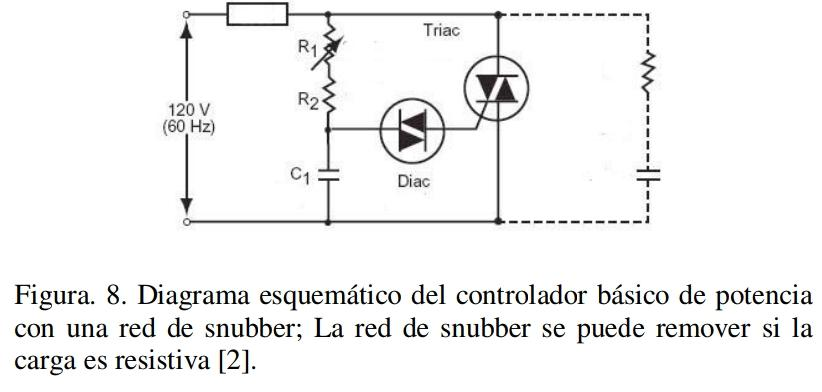
\includegraphics[scale=.5]{tarea2.jpeg}  $$
\\
\section{Bibliografia}
Concepcion Arelys, Octubre 2015, prezi.com, Mexico,\\ Recuperado de https://prezi.com/dh380hlercl/convertidores-ca-cd/
\end{document}